\chapter{First steps into probability}
Classical definition of probability:
\begin{equation*}
    P=\frac{\text{\#possible cases}}{\text{\#total cases}}
\end{equation*}
Only works with finite cases and equally probable cases.
\begin{definition}
An experiment is \textbf{random} if the outcome, given the initial configuration is uncertain.
\end{definition}
\begin{definition}
    $\Omega$ - \textbf{sample space}: the results, pairwise incompatible, of a random experiment.
\end{definition}
\begin{definition}
    $ \mathcal{P}(\Omega) $ - \textbf{power set} of $\Omega$: set of all subsets of $\Omega$. Cardinality is $ 2^{\#\Omega} $ (same cardinality of when we have n bits in binary (ex. if we have 4 bits then we have $2^4$ possible numbers), since we can think that 0 represents that we don't take the element, 1 if we take it).
\end{definition}
\section{Algebras and probability spaces}
\begin{definition}
    $ \mathcal{F} $ - \textbf{algebra}: family of subsets where the following holds:
    \begin{enumerate}
        \item $ \Omega \in \eff $
        \item if $ A \in \eff $ then $ A^C \in \eff $
        \item (finite case) if $ A, B \in \eff $, then $ A \cup B \in \eff $
    \end{enumerate}
\end{definition}
\vbox{
    Properties of $\eff$:
    \begin{enumerate}
        \item $\emptyset \in \eff$
        \item if $ A, B \in \eff $, then $ A \cap B \in \eff$
        \item if $ \{A_i\}^n_{i=1} \subseteq \eff$, then $\cap^n_{i=1}\, A_i \in \eff$
        \item if $A, B \in \eff $, then $A \setminus B \in \eff$
        \item if $A, B \in \eff$, then $A \,\Delta\, B \in \eff $ ($\Delta$ = elements present only in A or B, equivalent is $(A \cup B) \cap (A^C \cup B^C)$)
    \end{enumerate}
}
\begin{figure}[ht]
    \centering
    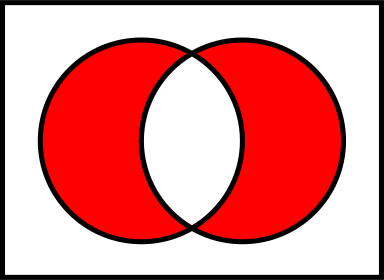
\includegraphics[width=0.25\textwidth]{images/Venn0110.png}
    \caption*{$A \,\Delta\, B$}
\end{figure}
\begin{definition}
    \sigal: same algebra as before, but also infinite unions are defined.
    Properties of \sigal s:
    \begin{enumerate}
        \item $ \Omega \in \eff $
        \item if $ A \in \eff $ then $ A^C \in \eff $
        \item for every countable family $ \{A_i\}^{+\infty}_{i=1} $ of subsets of $\Omega$, if all the sets $A_i$ are in \eff, then $\cup^{+\infty}_{i=1}\,A_i \in \eff$
    \end{enumerate}
\end{definition}
Since \sigal s accept also finite unions, all algebras are \sigal s.
\begin{example}
Difference between normal algebras and \sigal s.\\$\Omega = \symbb{N}$ $\aii$=\{$A \subseteq \symbb{N}$: $A$ is finite or $A^C$ is finite\}\\Let $A \in \aii$ and $B \in \aii$.\\If both finite, also union is finite => element of \aii. Now, let's look at numbers 2n. For any $n, 2n \in \aii$ as it is finite. But $\cup^{+\infty}_{i=1}\,2n \notin \aii$ => infinite union not contained in \aii => not a \sigal.
\end{example}
\begin{definition}
    \textbf{E - event}: every element $E \in \eff$ (\eff\, is a \sigal on $\Omega$). Singletons are elementary or atomic events.
\end{definition}
\begin{example}
    Let $\Omega=\{a, b, c\}$.\\Then we can define our \sigal{} as $\eff =\{\emptyset, \{a\}, \{b, c\}, \{a, b, c\}\}$
    \begin{itemize}
        \item $\{a\}$ is an atomic event
        \item $\{b\}$ is not an event
        \item $\{a, b, c\}$ is an event, but not atomic
    \end{itemize}
    Notice that we have checked all 3 properties of a \sigal: we have $\Omega$ and all complements.
\end{example}
\begin{definition}
    Given a set $\Omega$ and a \sigal{} \eff{}  on $\Omega$, the pair \borel{}is a \textbf{measurable space} or \textbf{Borel space}.
\end{definition}
\begin{definition}
    Given a measurable space \borel, a function $P: \eff \to \symbb{R}$ is a probability measure or probability function if it satisfies the following properties (Kolmogorov's axioms):
    \begin{enumerate}
        \item For every event E, $P(E) \ge 0$ (non negativity)
        \item $P(\Omega) = 1$ (normalization or total mass)
        \item given a countable family $\{E_i\}^{+\infty}_{i=1}$ of pairwise disjoint events, $P(\cup^{+\infty}_{i=1}E_i) = \sum_{i=1}^{\infty} P(E_i)$ ($\sigma$-additivity)
    \end{enumerate}
\end{definition}
The probability of E is the value P(E).
\begin{definition}
    Let $\Omega$ be a set, \eff{} a \sigal{} on $\Omega$, P a probability function on \eff. The triple \probspace{} is a \textbf{probability space}.
\end{definition}
Properties of probability measures:
\begin{enumerate}
    \item $P(\emptyset) = 0$
    \item if $E \in \eff \Rightarrow P(E^C) = 1 - P(E)$
    \item Let E, F events s.t. $E \subseteq F$. Then $P(E) \le P(F)$
    \item Image of any probability function is in unit interval [0, 1]
    \item \label{itm:incexl} $P(E \cup F) = P(E) + P(F) - P(E \cap F)$
    \item $P(E \cup F) \le P(E) + P(F)$
\end{enumerate}
\subsection{Inclusion-exclusion principle}
We can extend the notion of point \ref{itm:incexl} to the union of any number of sets. This is known as the inclusion-exclusion principle.
The idea is that we have to remove all elements that we have counted twice, add elements that we have removed three times etc.
\begin{figure}[ht]
    \centering
    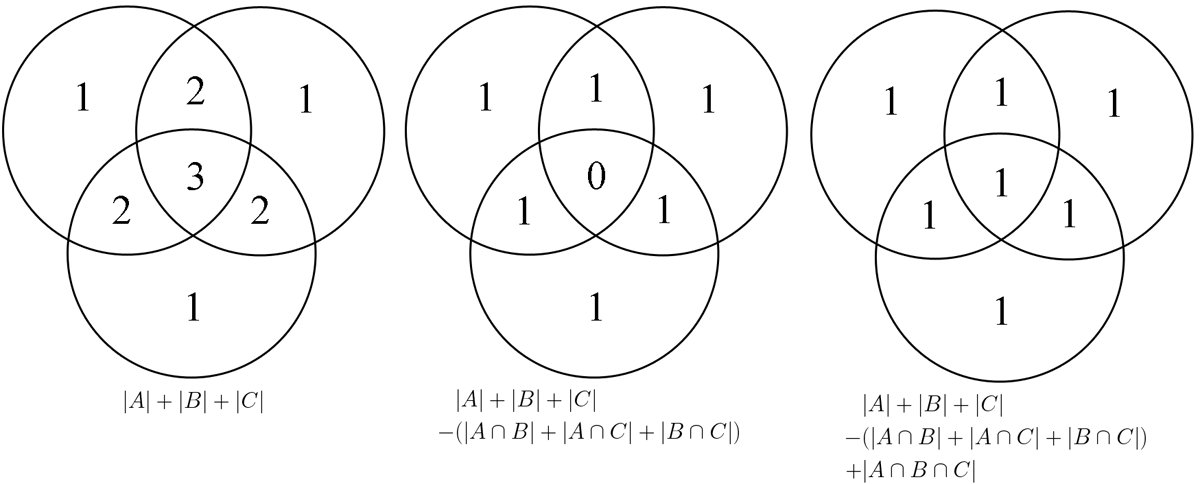
\includegraphics[width=0.8\textwidth]{images/Inclusion-exclusion-3sets.png}
    \caption*{Counting elements using the inclusion-exclusion principle with 3 sets}
\end{figure}
\begin{proposition}
    Let $\{E_i\}_{i=1}^n \subseteq \eff$  a finite family of sets. Then
    \begin{equation*}
        P\left(\bigcup_{i=1}^{n} E_i\right) = 
        \sum_{i=1}^nP(E_i) -
        \sum_{i<j}P(E_i \cap E_j) \footnote{$\sum_{i<j}=\sum_{i=1}^n\left(\sum_{j=i+1}^nP(E_i \cap E_j\right)$} +
        \sum_{i<j<k}P(E_i \cap E_j \cap E_k) +
        \cdots +
        (-1)^{n+1}P\left(\bigcap_{i=1}^nE_i\right)
    \end{equation*}
\end{proposition}
\begin{remark}
We can estimate from above (stopping at odd intersections) or below (stopping at even intersections). These are called Bonferroni bounds.
\end{remark}
\section{Conditional probability}
It is possible to extend the notion of probability spaces by adding conditions to our events.
\begin{definition}
    Given a probability space \probspace{} and two events E, F in \eff{} with $P(F) \neq 0$, we define the probability of E conditional to F ("E given F" per gli amici) as
    \begin{equation*}
        P(E|F) \coloneqq \frac{P(E \cap F)}{P(F)}
    \end{equation*}
\end{definition}
\begin{remark}
    $P(A^C|B)=1-P(A|B)$
\end{remark}
\textbf{WARNING!} $P(E|F)$ is not the same thing as $P(E \cap F)$! $P(E|F)$ denotes the probability of the intersection \underline{ONLY} on the F set, while $P(E \cap F)$ denotes the probability on the whole $\Omega$!
\begin{figure}[ht]
    \centering
    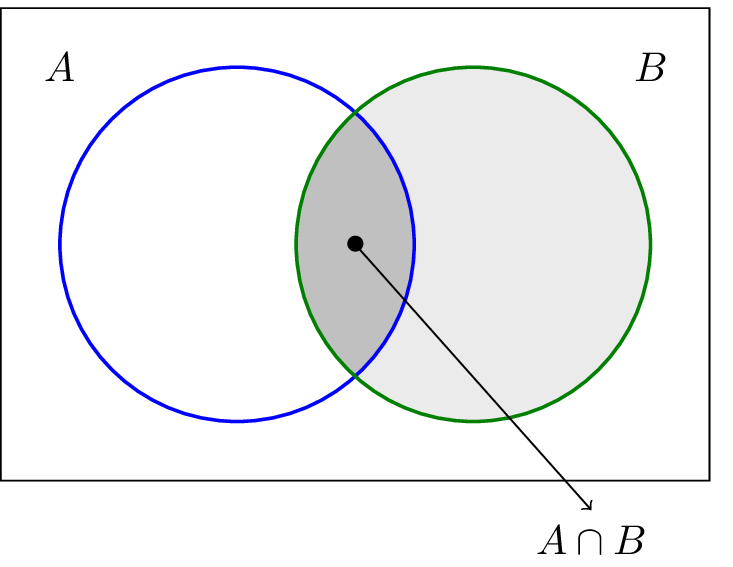
\includegraphics[width=0.4\textwidth]{images/conditional_b.png}
\end{figure}
\begin{remark}
    $P_F(\cdot) = P(\cdot{} | F) $ is a probability function, since it satisfies Kolmogorov axioms. Therefore also $P_F$ is a probability measure on the Borel space \borel, that is in general different from $P$.
\end{remark}
\begin{remark}
    Product rule
    \begin{equation*}
    \begin{gathered}
        P(E|F)=\frac{P(E \cap F)}{P(F)}\\
            \begin{aligned}
                P(E \cap F) & = P(E|F)P(F)\\
                & = P(F|E)P(E)
            \end{aligned}
    \end{gathered}
    \end{equation*}
\end{remark}
\subsection{Independence}
Let $E$ be the event that it rains tomorrow, and suppose that $P(E)=\frac{1}{3}$. Also suppose that I toss a fair coin; let $F$ be the event that it lands heads up. We have $P(F)=\frac{1}{2}$. Now I ask you, what is $P(E|F)$? What is your guess? You probably guessed that $P(E|F)=P(E)=\frac{1}{3}$. You are right! The result of my coin toss does not have anything to do with tomorrow's weather. Thus, no matter if F happens or not, the probability of E should not change. This is an example of two independent events. Two events are independent if one does not convey any information about the other.
\begin{definition}
    In a probability space \probspace{}, two events $E$, $F$ in \eff{} are \textbf{independent} (with respect to $P$) if the following holds: $P(E \cap F) = P(E) \cdot P(F)$. Sometimes the notation $E \perp F$ is used in this case.
\end{definition}
Now, let's first reconcile this definition with what we mentioned earlier, $P(E|F)=P(E)$. If two events are independent, then $P(E \cap F)=P(E)P(F)$, so
\begin{equation*}
    \begin{split}
    P(E|F) & = \frac{P(E \cap B)}{P(F)} \\
    & = \frac{P(E)P(F)}{P(F)} \\
    & = P(E).
\end{split}
\end{equation*}
An intuitive question we can ask ourselves is: is the probability of $E$ happening the same as $E$ happening after $F$? If that is the case, then the events are independent. Going back to the rain and coin case, the probability of getting heads is the same as the probability of getting heads after raining.
\begin{example}
    We have a $d6$. $E = \{2,4,6\}$ (getting an even number), $F = \{3, 6\}$ (getting a multiple of 3). Are these events independent?
    \begin{equation*}
        \frac{1}{2}\cdot\frac{1}{3} = \frac{1}{6} = P(E)P(F) = P(E \cap F) = \frac{1}{6}
    \end{equation*}
    Yes, they are. If we ask our "intuitive question", the probability of $F$ happening after $E$ is $\frac{1}{2}$, but also the probability of $E$ happening after $F$ is $\frac{1}{2}$, therefore the two events are independent.
\end{example}
Now we can extend this notion to more than 3 sets. For example, three events A, B and C are independent if all of the following conditions hold:
\begin{equation*}
    \begin{gathered}
        P(A \cap B) = P(A)P(B)\\
        P(A \cap C) = P(A)P(C)\\
        P(B \cap C) = P(B)P(C)\\
        P(A \cap B \cap C) = P(A)P(B)P(C)
    \end{gathered}
\end{equation*}
Now we can apply what we have seen with 3 sets to any number of sets.
\begin{definition}
    In a probability space \probspace, the events $E1,...,E_n$ are independent (with respect to P) if for any choice of indices (without repetition) $i_1,...,i_m$ in $\{1,...,n\}$ (with $m \le n$) it holds
    \begin{equation*}
        P\left(\bigcap_{j=1}^mE_{i_j}\right) = \prod_{j=1}^mP(E_{i_j}).
    \end{equation*}
\end{definition}
\subsection{Law of total probability/factorisation formula}
\begin{theorem}
    Let \probspace, $\{E_i\}_{i=1}^n$ disjoint, $P(E_i)>0 \; \forall i$, $\quad \bigcup_{i=1}^nE_i=\Omega$
    \begin{equation*}
        \forall E \in \eff \quad P(E) = \sum_{i=1}^n P(E \cap E_i) = \sum_{i=1}^n P(E|E_i)P(E_i)
    \end{equation*}
\end{theorem}
Using a Venn diagram, we can pictorially see the idea behind the law of total probability. In the next figure, we have
\begin{equation*}
    \begin{gathered}
    A_1 = A \cap B_1\\
    A_2 = A \cap B_2\\
    A_3 = A \cap B_3\\
    \end{gathered}
\end{equation*}
As it can be seen from the figure, $A_1$, $A_2$, and $A_3$ form a partition of the set A, and thus by the third axiom of probability
\begin{equation*}
    P(A)=P(A_1)+P(A_2)+P(A_3).
\end{equation*}
\begin{figure}[ht]
    \centering
    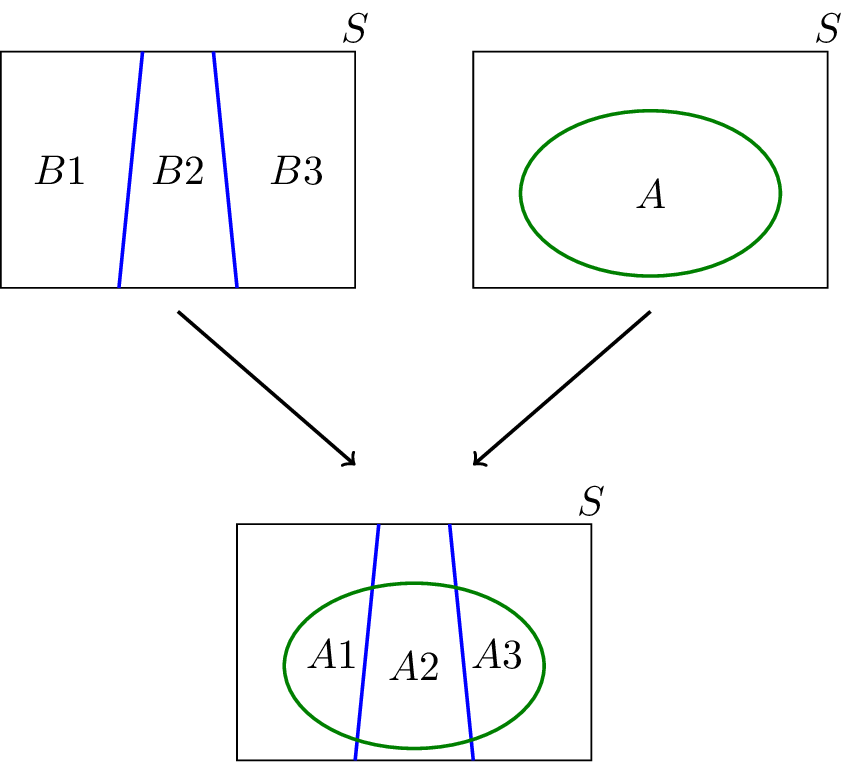
\includegraphics[width=0.5\textwidth]{images/total.png}
    \caption*{Law of total probability}
\end{figure}
\subsection{Bayes theorem}
\begin{theorem}
Let \probspace{} be a probability space and $E, F$ two events, both with non-zero probability. Then
\begin{equation*}
    P(E|F)=\frac{P(F|E)}{P(F)} \cdot P(E).
\end{equation*}
Proof:
\begin{equation*}
    P(E|F)=\frac{P(E \cap F)}{P(F)}=\frac{P(E \cap F)}{P(E)}\cdot\frac{P(E)}{P(F)}=\frac{P(F|E)\cdot P(E)}{P(F)}
\end{equation*}
\end{theorem}